\subsection{An exact two-generator example with hourly ramps}
Keep every fleet constraint and continuous charging choice from
Section~\ref{sec:exact}. Generation now spans the consecutive hours
$[1,2]$, $[2,3]$, and $[3,4]$: the fleet load is
$L=(x,0,30-x)$ and background demand is $b=(0,15,0)$. The middle hour,
when service B operates, cannot be omitted from an hourly ramp model.
Both generators start at zero; no terminal generation level is imposed.
Costs are declared synthetic hourly offers, with no fixed commitment costs.
Generator A has marginal costs $(7,5,1)$ and capacities $(10,15,15)$;
generator B has costs $(6,5,5)$ and capacities $(10,15,30)$.
A's initial upward limit is 10 and its two subsequent hourly upward limits
are 5. All downward limits and B's upward limits are 30. Power and energy
numbers coincide in these one-hour intervals.

Background supply costs $H(b)=75$. Let $a,m,z$ denote A's early, middle
and terminal outputs. On the full feasible fleet interval $0\le x\le10$,
subtracting the baseline leaves $150+x+a-4z$. The two ramps and terminal
capacity imply $z\le\min(15,a+10)$, attained with $m=a+5$ for every
$a\in[0,x]$. Minimizing over $a$ therefore gives the exact supply value
\begin{equation}\label{eq:ramp-value}
 G(x,0,30-x)=
 \begin{cases}110-2x,&0\le x\le5,\\95+x,&5\le x\le10.\end{cases}
\end{equation}
The one-bus plan costs $7+G(10,0,20)=112$; the best two-bus plan costs
$14+G(5,0,25)=114$. The complete-fleet hull retains the operating-cost
boundary $14-0.7x$, giving
\begin{equation}\label{eq:ramp-gap}
 D_G=112,\qquad CH_G=\frac{221}{2}=110.5,\qquad D_G-CH_G=\frac32.
\end{equation}
The minimizing mixture gives equal weight to the one-bus load $(10,0,20)$
and the two-bus load $(0,0,30)$. At its mean $(5,0,25)$, dispatch is
A $=(5,10,15)$ and B $=(0,5,10)$, with both of A's hourly upward ramps
binding (Figure~\ref{fig:ramp-example}).

At that mean the exact set of balance prices is
$p=(s,5,5)$, $3\le s\le6$. Positive B output fixes the last two prices;
A's stationarity gives equal ramp rents $7-s$ and terminal-capacity rent
$s-3$, while B's unused early output requires $s\le6$. Selecting
$p^*=(5.7,5,5)$ makes the two supporting fleet plans tie at private cost
164. Its generator dual supplies the global cut
$G(L)\ge(p^*)^\top L-53.5$, tight at the mean. Thus the dual lower bound
is $164-53.5=110.5$, equal to the mixture upper bound. This derivation is
independent of the quadratic example's prices.

The physical one-bus optimum has the unique dispatch price $(6,5,5)$ and
regret 3. The physically feasible two-bus plan at the kink $x=5$ instead
has a price-dependent regret: $32-5s$ for $3\le s\le5.7$, and $5s-25$
for $5.7\le s\le6$. Its smallest admissible regret is 3.5, attained at
$s=5.7$, equal to its physical cost minus $CH_G$. This illustrates why a
nonsmooth supply model needs a declared price selection or a test over
the admissible set.

Relaxing only A's two inter-hour upward limits from 5 to 30 gives
$G_0(x,0,30-x)=90+x$. Both the physical and hull minima then equal 104,
attained by the two-bus plan with $x=0$. These controlled synthetic cases
isolate the change in the supply constraints; they are not measurements of
price-support failure in a public timetable. Small LP solutions independently
check dispatch, balance prices and hull values, while the affine branch
derivation and rational dual certificate establish the exact claims.

\begin{figure}[t]
\centering
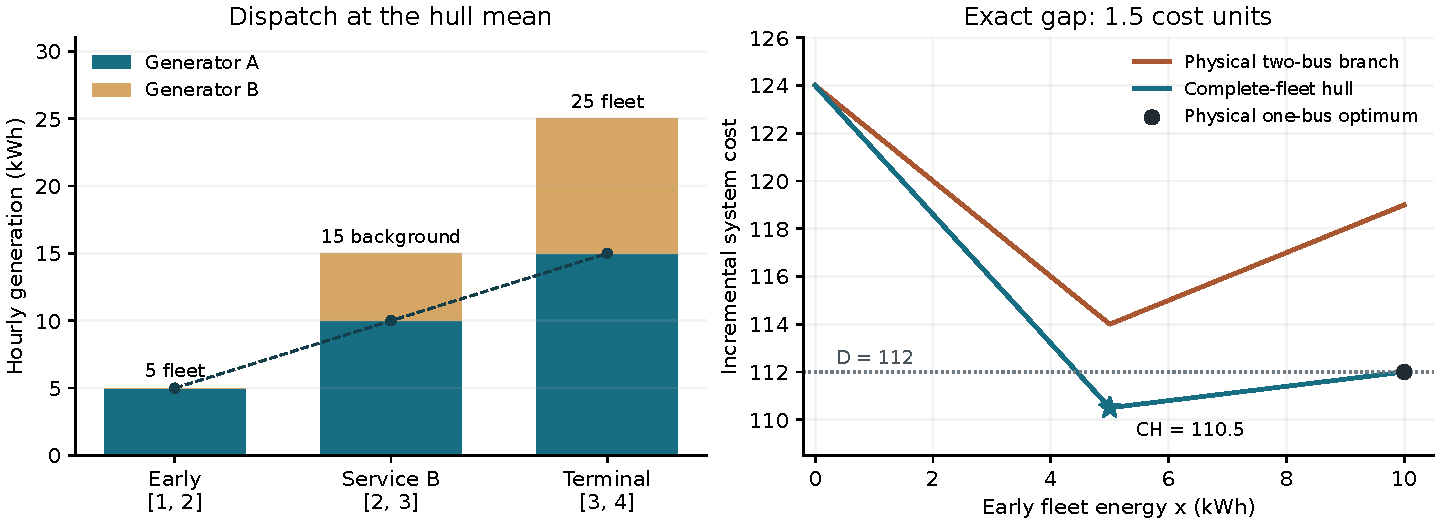
\includegraphics[width=\linewidth]{figures/ramped_generation_example.pdf}
\caption{The hourly generation example. Left: generation serving the hull
mean; the middle hour serves only background demand, and A rises by its
5-unit limit in each interval. Right: physical two-bus and hull costs over
the full continuous charging interval, with the one-bus optimum marked
separately. All costs and offers are synthetic.}
\label{fig:ramp-example}
\end{figure}
